\uuid{iohc}
\exo7id{5049}
\titre{exo7 5049}
\auteur{quercia}
\organisation{exo7}
\datecreate{2010-03-17}
\isIndication{false}
\isCorrection{true}
\chapitre{Surfaces}
\sousChapitre{Surfaces paramétrées}
\module{Géométrie}
\niveau{L2}
\difficulte{}

\contenu{
\texte{
On considère la surface ${\cal S}$ d'équations paramétriques :
$\begin{cases} x = \rho\cos\theta\cr
         y = \rho\sin\theta\cr
         z = f(\rho,\theta)\cr \end{cases}$
où $f$ est une fonction de classe $\mathcal{C}^1$.
}
\begin{enumerate}
    \item \question{Donner l'équation du plan tangent à ${\cal S}$ en un point $M(\rho,\theta)$.}
\reponse{$\left(\sin\theta\frac{\partial f}{\partial \theta} -\rho\cos\theta\frac{\partial f}{\partial \rho}\right)x
             -\left(\cos\theta\frac{\partial f}{\partial \theta} +\rho\sin\theta\frac{\partial f}{\partial \rho}\right)y
             + \rho z = \rho f - \rho^2\frac{\partial f}{\partial \rho}$.}
    \item \question{Déterminer $f$ de sorte que, le long d'une ligne $\theta = \text{cste}$,
    le plan tangent coupe $Oz$ en un point fixe.}
\reponse{$f-\rho\frac{\partial f}{\partial \rho} = a(\theta)
              \Rightarrow  f(\rho,\theta) = a(\theta) + b(\theta)\rho$.}
    \item \question{Exemple : $f(\rho,\theta) = \theta$. Dessiner la surface ${\cal S}$.}
\reponse{$$
\centerline{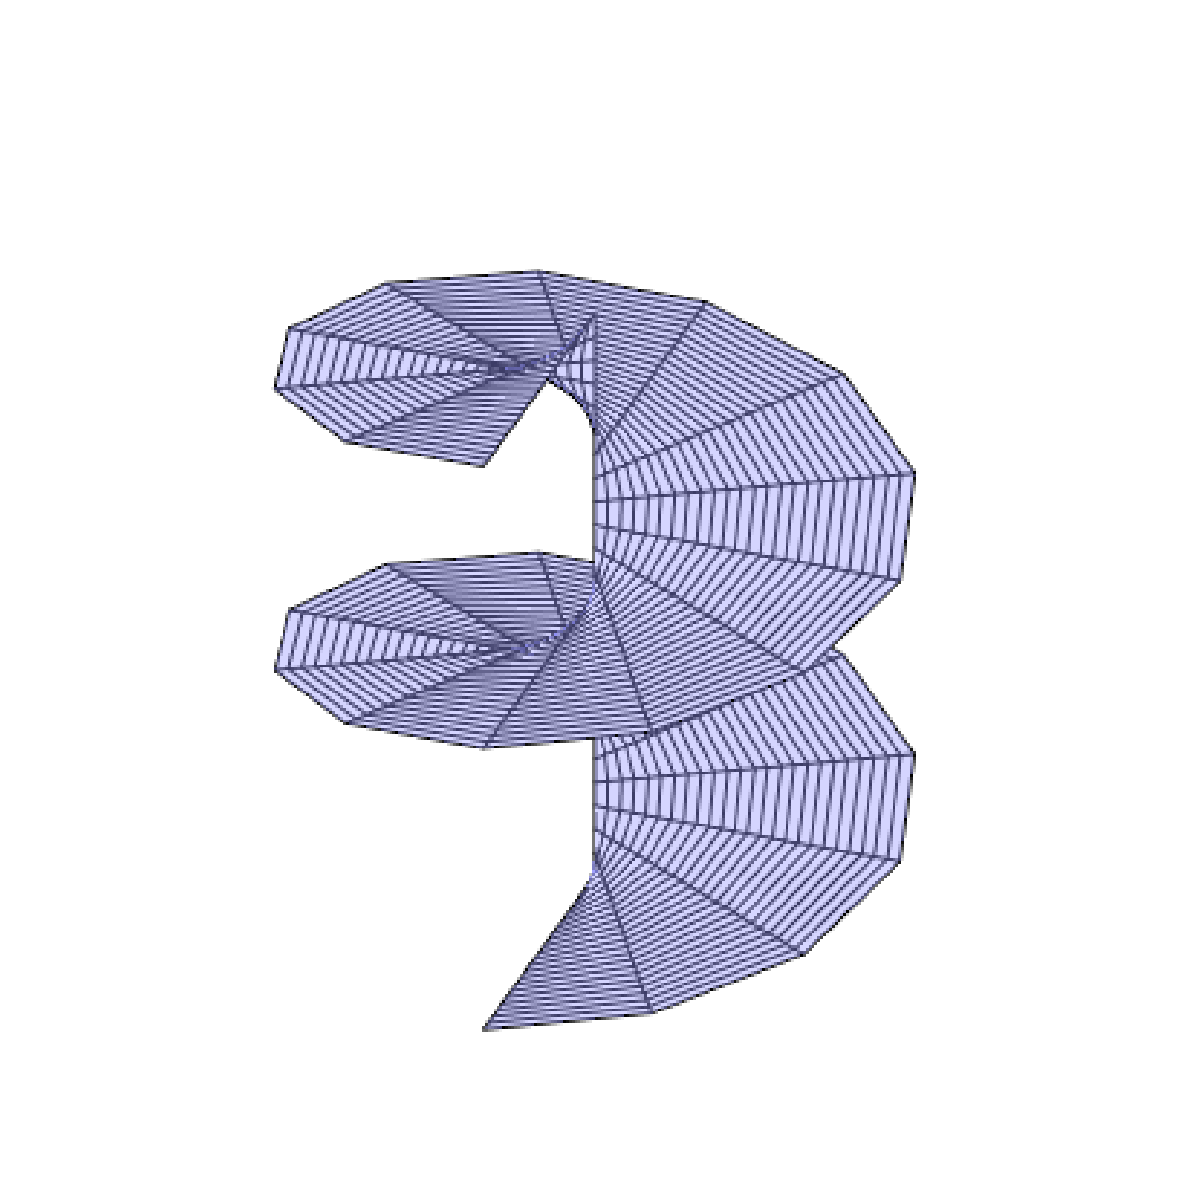
\includegraphics[height=6cm]{../images/img005049-1}}
$$
  % \mapleplot{ x := r*cos(t); y := r*sin(t); z := t;    plot3d([x,y,z],r=0..2,t=0..4*Pi,style=hidden,color=black,orientation=[20,60]);   }}
\end{enumerate}
}
